\documentclass[french]{beamer}

% Animations
\usepackage{xmpmulti}
%Arbre pour goal babling
\usepackage{tikz}
\usetikzlibrary{trees}
%Centrer verticalement les tableaux
\usepackage{array}
\usepackage{changepage}
%Coloration des frames avec mathrice.sty
\usepackage{mathrice}
\usepackage{tikz}
\usepackage{caption}
\usepackage{graphicx}
\graphicspath{{./graphics/}}

% Enlève les boutons de navigation des frames
\beamertemplatenavigationsymbolsempty

% Ajoute le logo FST sur chaque slides
\setbeamertemplate{background}{
    \begin{tikzpicture}[remember picture,overlay]
    \node[anchor=south west] at (current page.south west) {
\includegraphics[height=1cm]{Logo_FST.jpg}};
\end{tikzpicture}}

% Numérotation des slides
\setbeamertemplate{footline}[frame number]

% Frame section dans un rectangle bleu foncé
\AtBeginSection[]{
  \begin{frame}
    \vfill
    \centering
    \begin{beamercolorbox}[sep=8pt,center,shadow=true,rounded=true]{title}
        \usebeamerfont{title}\insertsectionhead\par
    \end{beamercolorbox}
    \vfill
  \end{frame}
}

% Page de garde
\title{Comment découvrir son corps?}
\author{Lucas SCHWAB}
\date{Mars - Août 2019}

%%%%%%%%%%%%%%%%%%%%%%%%%%%%%%%%%%%%
%%%%%%%%%%%%% Document %%%%%%%%%%%%%
%%%%%%%%%%%%%%%%%%%%%%%%%%%%%%%%%%%%
\begin{document}

% Page de garde
\begin{frame}
    \begin{center}
        \begin{beamercolorbox}[sep=8pt,center]{title}
            \usebeamerfont{title}
            \Huge \textbf{Stage Master 2}

            \huge Comment découvrir son corps?
        \end{beamercolorbox}
        \vfill

        Lucas SCHWAB

        \vfill

        Encadrants:

        Amine BOUMAZA
        \&
        Alain DUTECH
    \end{center}
\end{frame}

%-----------------------------------

% Sommaire
\begin{frame}
    \hfill
    \parbox[t]{.88\textwidth}{
        \begin{minipage}[c][0.75\textheight]{0.88\textwidth}
        \tableofcontents
        \end{minipage}
    }
    % Introduction
    %     Contexte
    %     Babling
    % Travail Realise
    %     Principe
    %     Algorithmes
    % Apprentissage
    %     Processus
    %     Resultats
    % Conclusion
\end{frame}

%###################################
\section{Introduction}

%###
\subsection{Contexte}
% Le but est d'apprendre à un robot à découvrir son corps. Le robot vit dans le monde réel, on lui donne une position à atteindre, on ne connait pas les angles à lui donner. Trouver la commande à exécuter pour atteindre un but donnée est le rôle de la cinématique inverse.

%-----------------------------------

% Comment calculer, cinématique inverse
\begin{frame}
    \frametitle{Cinématique Inverse}
    % Il y a plusieurs espaces particuliers pour un robot. On a l'espace de travail qui, dans le cas d'un bras robotique, est tout l'espace que peut atteindre le robot. Une position dans cet espace est caractérisée par les coordonnées cartésiennes de l'effecteur. On a ici l'espace de configuration, qui est tous les angles que peuvent prendre les moteurs du robot. Une position ici est caractérisée par les angles de chacun des moteurs.
    % Pour passer d'une position dans l'espace de configuration à une position dans l'espace de travail, on utilise la cinématique directe.
    % Dans l'autre sens, pour obtenir la pose associée permettant d'atteindre une position dans l'espace de travail, on utilise la cinématique inverse.

    % Lorsqu'un robot ne permet pas de redondance, done atteindre la même position avec plusieurs poses différentes, il est possible d'avoir la cinématique inverse de manière déterministe. Il existe une solution analytique permettant de trouver quelle sera la commande à donner pour atteindre une position demandée.
    % Si le robot est redondant, il n'y as pas de solution analytique pour le modèle inverse comme c'est le cas pour Poppy Ergo Jr. Pourtant il existe une bibliothèque appellée Ikpy qui propose une cinématique inverse. Celle ci est calculée en utilisant un algorithme d'optimisation L-BFGS, en donnant chaques angles des moteurs à optimiser, et la distance entre la position de l'effecteur (obtenue avec la cinématique directe) et le but à minimiser.

    % Je vais explorer une autre manière de générer une cinématique inverse.
    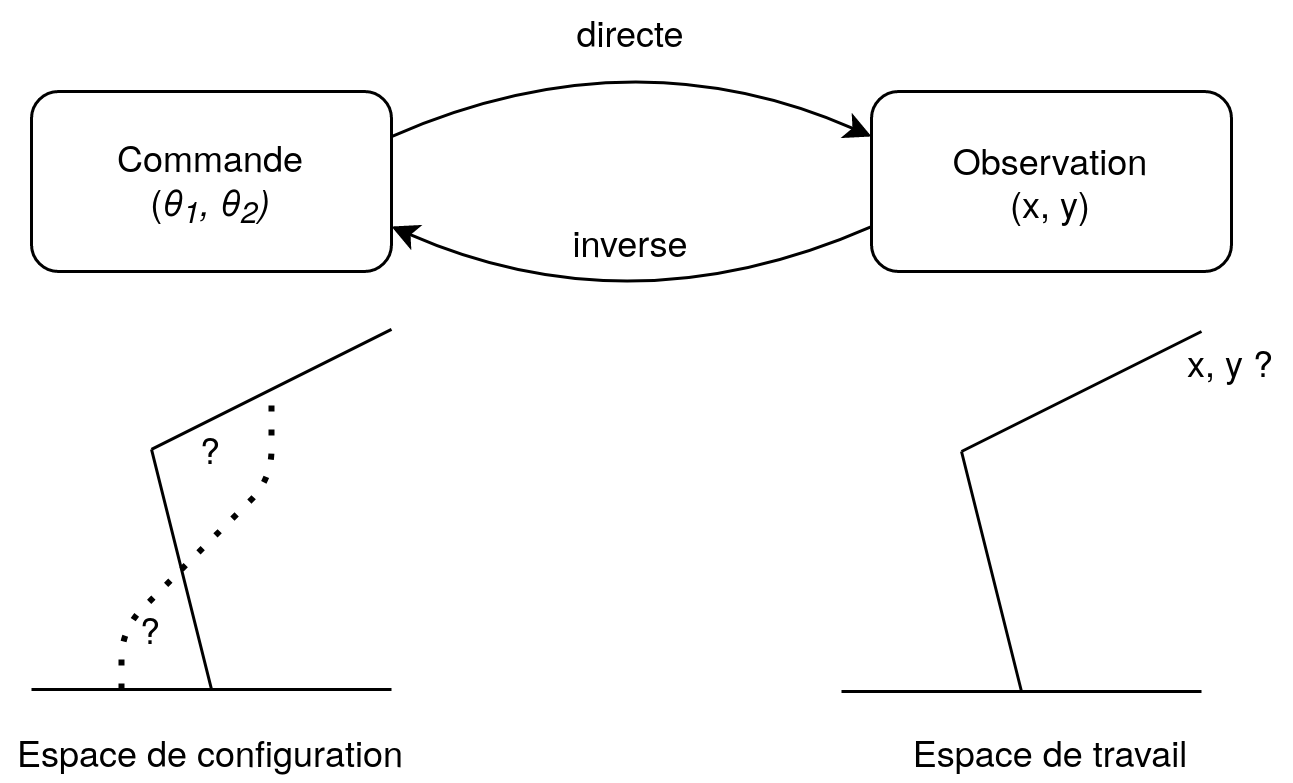
\includegraphics[width=\textwidth]{Modelisation_Diagram_w_espaces.png}
\end{frame}

%###
\subsection{Babling}

% Mon travail -> Babling & Ergo
\begin{frame}
    \frametitle{Poppy Ergo Jr}

    % Le robot utilisé pendant ce stage est le Poppy Ergo Jr. Il est composé d'une base et d'un effecteur en forme d'abat-jour, ainsi qu'une suite de moteur et de sections rigides. J'ai utilisé une méthode de babillage (babling en anglais) pour générer une cinématique inverse pour ce robot.
    
    % La méthode babling s'inspire du processus développementale des systèmes biologiques. Cad qu'il s'inspire de la manière dont un nouveau né se développe    e comment son corps bouge.
    \center
    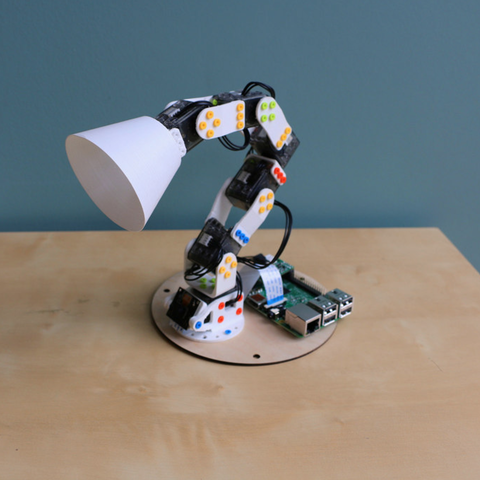
\includegraphics[width=0.5\textwidth]{Poppy_Ergo_Jr.png}
    % poppy
    % mise en place du Babling
\end{frame}

%-----------------------------------

% Babling: inspiration du processus développementale
\begin{frame}
    \frametitle{Babling}
    % Le principe du babling consiste à acquérir de l'expérience lors d'une étape qui s'apparente à l'enfance. Cette expérience sera ensuite utilisée comme une cinématique inverse. L'apprentissage consiste donc à générer de l'expérience et à l'utiliser pour créer une cinématique inverse.

    \center
    \begin{tabular}[]{m{0.4\textwidth} m{0.4\textwidth}}
        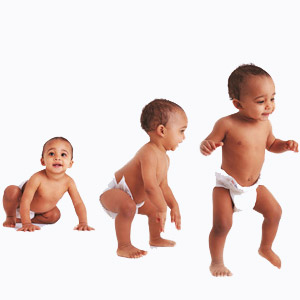
\includegraphics[width=0.4\textwidth]{baby-walk.jpg}  &  \center Processus Développemental
    \end{tabular}
\end{frame}

%###################################
\section{Travail Réalisé}
% Je vais donc vous présenté le travail que j'ai réalisé pour créer cette cinématique inverse.

%###
\subsection{Principe}

% Expliquer la fonction f: X -> Q
\begin{frame}
    \frametitle{Cinématique Inverse}
    % La cinématique inverse est une fonction qui prend un effet en paramètre, ici une position cartésienne. Elle retourne une commande, les angles pour les moteurs.
    % Cette fonction est basée sur l'expérience du robot, acquise de manière autonome et aléatoire. Je vais caractériser cette expérience par un catalogue, qui contient une liste de commande et des effets associés


    \center
    \begin{tabular}{m{0.4\textwidth} m{0.5\textwidth}}
        \Large
        \begin{align}
            f: X \rightarrow Q \nonumber
        \end{align}

        &

        \center
        Catalogue

        \begin{tabular}{||c | c ||}
            \hline
            Commande (Q) & Effet (X) \\
            \hline
            $\theta_{a1}, \theta_{b1}, ...$ & x, y, z\\
            $\theta_{a2}, \theta_{b2}, ...$ & x, y, z\\
            $\theta_{a3}, \theta_{b3}, ...$ & x, y, z\\
            ... & ...\\
            \hline
        \end{tabular}
    \end{tabular}


    % Effet, mouvement
    % Aleatoire
    % Fo : Q..., effet
\end{frame}

%-----------------------------------

% Comment construire F
\begin{frame}
    % Pour construire ce catalogue, je vais utiliser plusieurs méthode de babling. Premièrement le Motor Babling, pour babillage moteur. On donne une pose totalemet aléatoire au robot, et on ajoute la commande et son observation au catalogue.
    % Ensuite je vais parler du Goal Babling qui possède plusieurs variante. Le Goal babling, pour babillage par but, consiste à générer un but qui permet de diriger l'apprentissage. Je vais ensuite prendre l'observation dans le catalogue la plus proche de ce but, et la perturber, cad la modifier aléatoirement, afin de générer une nouvelle observation.
    % Je vais donc présenter les différents algorithmes.

    \tikzstyle{every node}=[draw=black,thick,anchor=west]
    \tikzstyle{selected}=[draw=red,fill=red!30]
    \tikzstyle{optional}=[dashed,fill=gray!50]
    \begin{tikzpicture}[
        grow via three points={one child at (0.5,-0.7) and
        two children at (0.5,-0.7) and (0.5,-1.4)},
        edge from parent path={(\tikzparentnode.south) |- (\tikzchildnode.west)}]
            \node {Cinématique Inverse}
            child { node [selected] {Babling}
                child { node {Motor Babling} }
                child { node {Goal Babling} }
            }
            child [missing] {}
            child [missing] {}
            child { node { Solution Analytique } }
            child { node { Optimisation } }
            child { node { ... } };
    \end{tikzpicture}
    



    % Motor Babling
    %Goal Babling : plusieurs variantes
\end{frame}

%###
\subsection{Algorithmes}

% Motor Babling
\begin{frame}
    \frametitle{Motor Babling}
    % Le Motor babling, qui consise à générer une pose aléatoire uniformément sur l'espace de configuration du robot, et ajoute cette commande au catalogue.
    % Comme la pose est générée uniformément dans l'espace de configuration, tout l'espace de travail a une probabilité non nul d'être couvert par le catalogue. Cependant, il existe des zones plus facile à atteindre pour le robot. En générant une pose aléatoire, le robot a plus de chance d'être replié sur lui-même que d'être tendu. L'espace de travail n'est donc pas uniformément exploré.
    %C'est pour cela que j'ai utilisé une autre méthode, le Goal Babling.

    \begin{tabular}{c c c}
        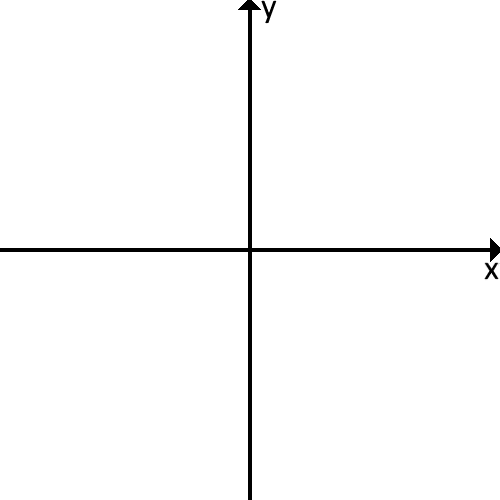
\includegraphics[width=.28\textwidth]{poppy_motor_babling/frame-0.png}
        &
        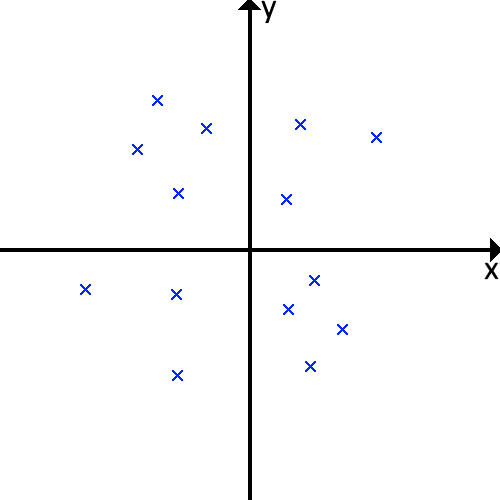
\includegraphics[width=.28\textwidth]{poppy_motor_babling/frame-1.png}
        &
        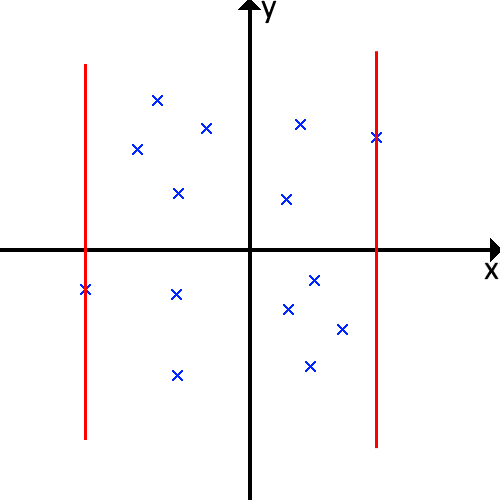
\includegraphics[width=.28\textwidth]{poppy_motor_babling/frame-2.png}
        \\
        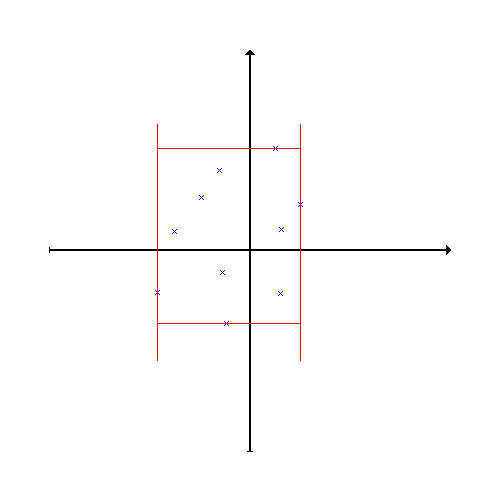
\includegraphics[width=.28\textwidth]{poppy_motor_babling/frame-3.png}
        &
        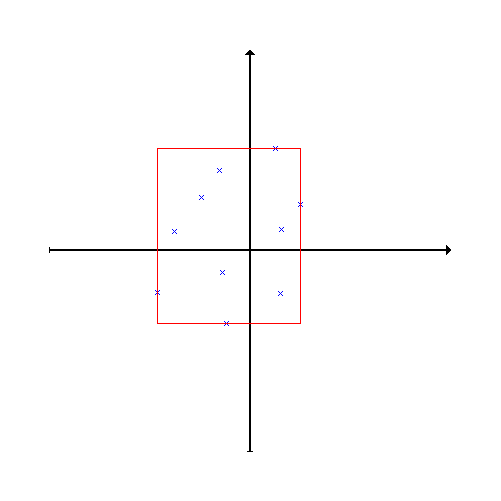
\includegraphics[width=.28\textwidth]{poppy_motor_babling/frame-4.png}
        &
        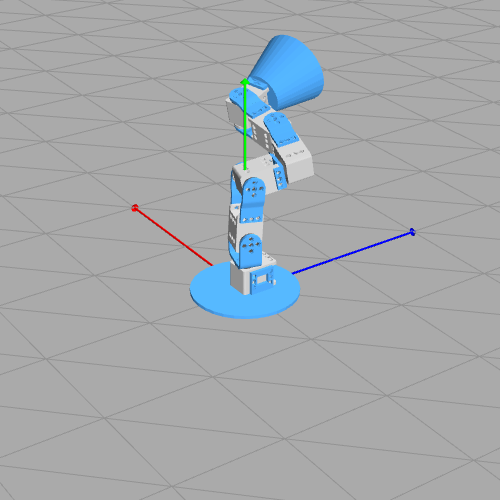
\includegraphics[width=.28\textwidth]{poppy_motor_babling/frame-5.png}
    \end{tabular}

    % Algorithme

\end{frame}

%-----------------------------------

% Goal Babling: Agnostique
\begin{frame}
    \frametitle{Agnostic Goal Generator}
    % L'agnostic goal generator est une instantiation du goal babling. La génération de but se fait de manière agnostic, cad il est impossible de tout connaitre, comme les limites de l'espace de l'espace du travail du robot.
    % Lors du remplissage du catalogue, je vais retenir les positions extrêmes rencontrées. cad le minimum et maximum sur chacun des axes. Cette zone est une estimation de l'espace de travail du robot. Afin d'avoir de l'exploration, dans le cas où la portée du catalogue est une sous-estimation de l'espace de travail, je vais agrandir cette zone et y générer un but.
    
    \center
    \multiinclude[<+>][format=png, graphics={width=.7\textwidth}]{agnostic_gg/frame}

\end{frame}

%-----------------------------------

% Goal babling: Frontier
\begin{frame}
    \frametitle{Goals on Grid \& Frontier}
    % L'estimation de l'espace de travail faite par l'Agnostic Goal Generator n'est qu'un cube grossier. Afin de mieux l'approcher, j'ai discrétisé l'espace. J'ai donc une grille, où il me suffit de noter quelles cellules sont visitées par le catalogue. J'obtiens ainsi une approximation de la portée du robot avec une résolution que je peux choisir.
    % L'algorithme Goals on Grid peut donc générer un but dans n'importe quelle cellule de cette grille. Une probabilité p permet de contrôler l'exploration de l'algorithme. Avec une probabilité p, je vais générer un but dans une cellule non explorée afin d'augmenter la portée du catalogue. Et avec une probabilité 1-p, je vais générer une but dans une cellule déjà explorée. Ainsi, si le catalogue a déjà remplis l'espace de travail, je peux continuer à générer des but pertinents. 

    % La selection d'une cellule non explorée est le rôle de l'algorithme Frontier.
    % Afin de trouver quelle est la frontière des cellules visités, je pars d'une observation du catalogue choisie aléatoirement. Je choisis ensuite une direction, aléatoirement. Je vais suivre cette direction à partir de l'observation jusqu'à rencontrer une cellule non visitée. C'est dans celle-ci que le prochain but sera généré.


    \center
    \multiinclude[<+>][format=png, graphics={width=.7\textwidth}]{frontier/frame}

    % La grille etc, chercher la frontière
\end{frame}



%###################################
\section{Apprentissage}
% Maintenant que j'ai décris les algorithme, je vais maintenant décrire le déroulement d'un apprentissage


%###
\subsection{Processus}

% Experience - lancer - mesurer
\begin{frame}
    \frametitle{Expérience}
    % Une execution d'algorithme est une expérience qui contient certains paramètres. Je vais lancer une expérience et mesurer les résultats.
    % La mesure des résultats se fait en calculant la couverture et la précision de mon catalogue.
    % Le catalogue ne contient qu'un nombre fini d'entrées. Afin de couvrir l'espace réel qui est continue, j'utilise une interpolation des 3 observations les plus proches du but.
    
    Choisir paramètres $\Rightarrow$ Lancer apprentissage $\Rightarrow$ Mesurer résultat
\end{frame}

\begin{frame}
    \frametitle{Couverture}
    % Pour connaitre la couverture d'un catalogue, j'ai choisis de prendre le volume de l'enveloppe convexe de toutes les observations du catalogue. J'ai aussi calculé le volume occupé par toutes les cellules visitées. J'ai le volume de l'enveloppe convexe, et j'ai le remplissage de ce volume.
    
    \center
    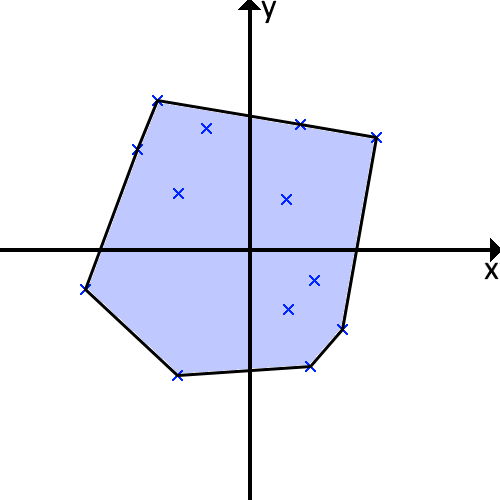
\includegraphics[width=.45\textwidth]{couverture/volu-1.png}
    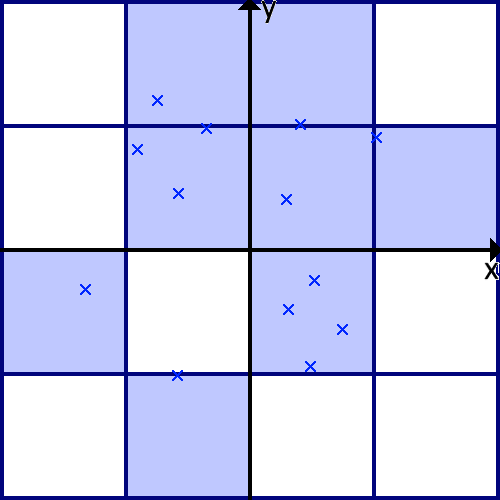
\includegraphics[width=.45\textwidth]{couverture/remp-1.png}


    Enveloppe convexe remplissage
\end{frame}

\begin{frame}
    \frametitle{Précision}

    % Pour connaitre maintenant la précision du catalogue, j'ai généré une liste de but théoriquement atteignable, cad à la portée du robot. Je mesure ensuite l'erreur de la cinématique inverse pour exprimer la précision. L'erreur c'est la distance entre le but et le résultat de la cinématique inverse.
    % J'ai aussi utilisé Ikpy, la bibliothèque présente pour controller le robot, pour atteindre tout les buts de cette liste. J'obtiens une autre liste, cette fois-ci d'observation. Cad que ces points ne sont pas seulement théoriquement atteignable, ils sont atteignables.
    
    \begin{tabular}{c c}
        Vue de face & Vue du dessus
        \\
        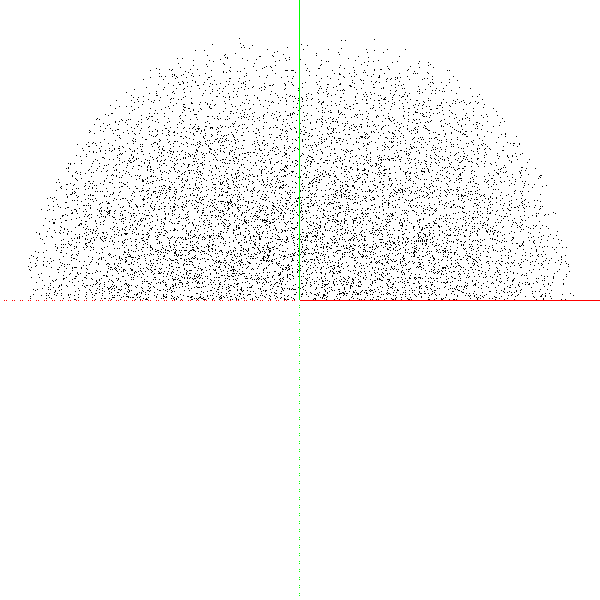
\includegraphics[width=.45\textwidth]{goal_list_front.png} &
        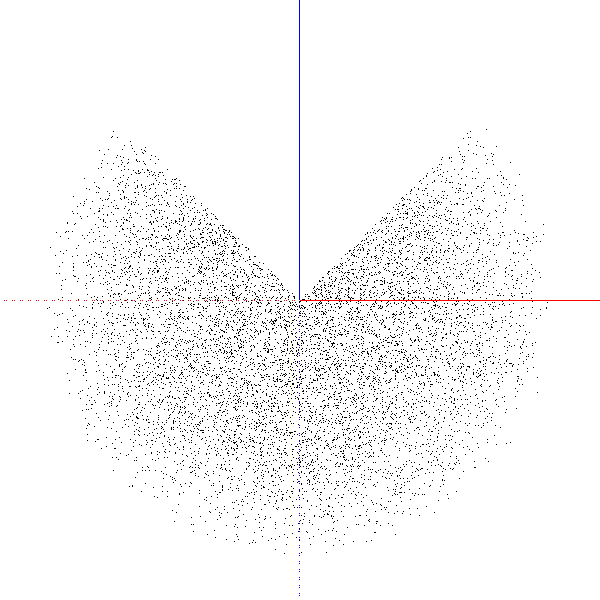
\includegraphics[width=.45\textwidth]{goal_list_top.png}
    \end{tabular}

    % L'apprentissage se résume à préparer une expérience, donc choisir les paramètres. Puis démarrer l'expérience et mesurer le résultat. Et ce, pour tous les paramètres des algorithmes.




    % Quelles mesures: couverture / précision
    % Décrire comment mesurer
    % Décrire qu'ils faut lancer pour des paramètres différents
    % Interpolation?
\end{frame}

%###
\subsection{Résultats}
% Je vais maintenant présenter les résultats de mon apprentissage

% Resultats Motor Babling
\begin{frame}
    \frametitle{Motor Babling}
    \begin{tabular}{c c}
        Couverture (volume) & Précision (distance liste ikpy)
        \\
        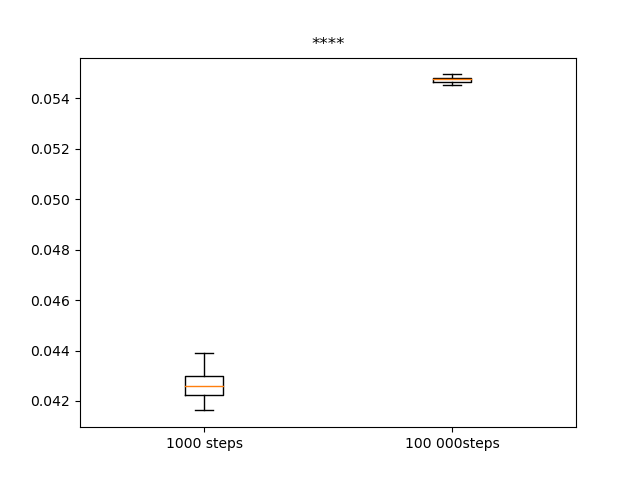
\includegraphics[width = 0.45\textwidth]{1mb_1k-100kstep_couver.png} &
        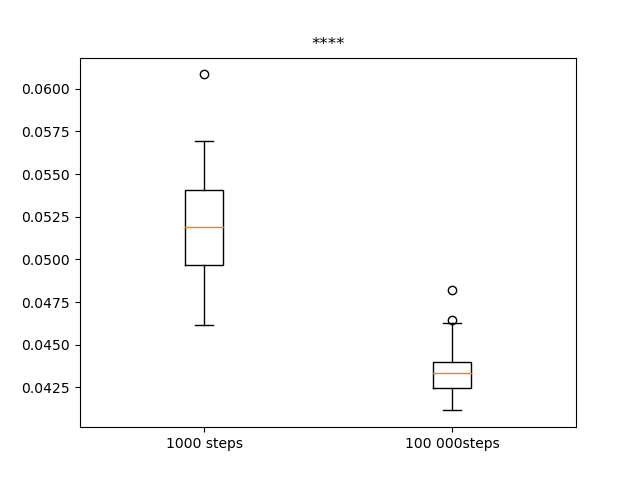
\includegraphics[width = 0.45\textwidth]{1mb_1k-100kstep_moy_ik.png}
    \end{tabular}
\end{frame}

%-----------------------------------

% Resultats Goal Babling
\begin{frame}
    \frametitle{Goal Babling}
    \begin{tabular}{c c}
        Couverture (volume) & Précision (distance liste ikpy)
        \\
        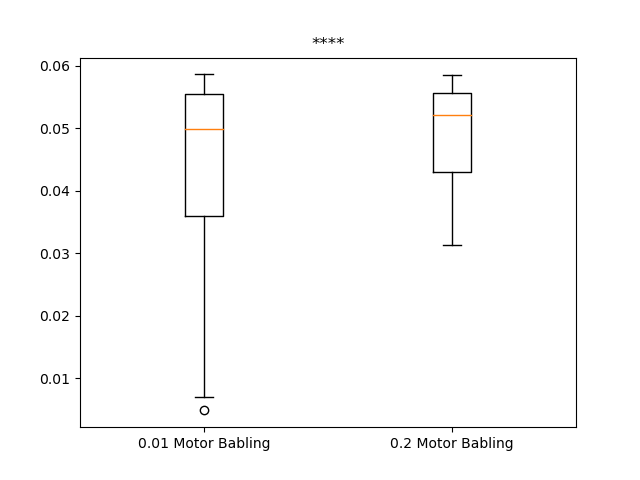
\includegraphics[width = 0.45\textwidth]{0.2-.01mb_couver.png} &
        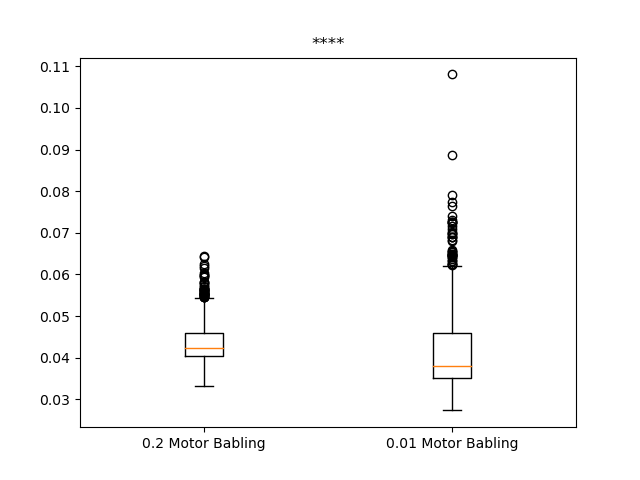
\includegraphics[width = 0.45\textwidth]{0.2-.01mb_moy_ik.png}
    \end{tabular}
\end{frame}

%-----------------------------------

% Résultats Agnostique
\begin{frame}
    \frametitle{Agnostic Goal Generator}
    \begin{tabular}{c c}
        Couverture (volume) & Précision (distance liste ikpy)
        \\
        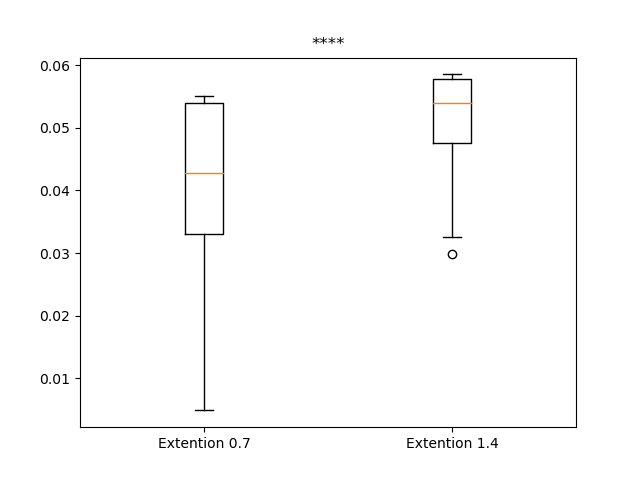
\includegraphics[width = 0.45\textwidth]{Agn_.7-1.4exp_couver.png} &
        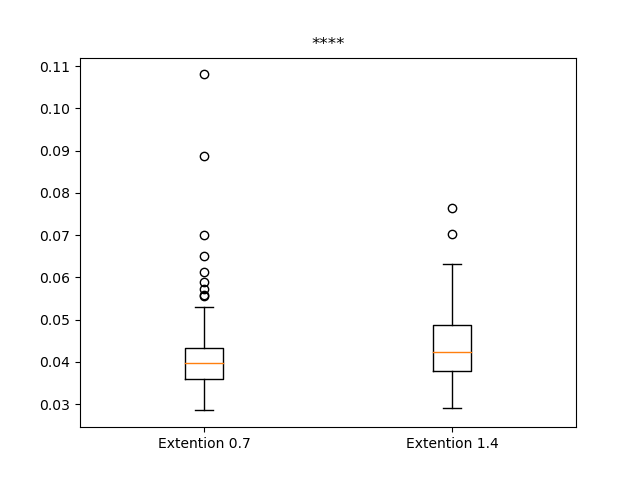
\includegraphics[width = 0.45\textwidth]{Agn_.7-1.4exp_moy_ik.png}
    \end{tabular}
\end{frame}

%-----------------------------------

% Résultats Frontier
\begin{frame}
    \frametitle{Frontier}
    \begin{tabular}{c c}
        Couverture (volume) & Précision (distance liste ikpy)
        \\
        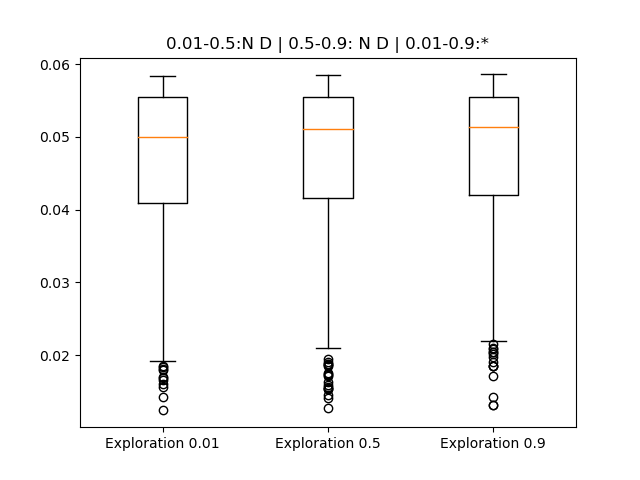
\includegraphics[width = 0.45\textwidth]{Fro_.01-.5-.9pexp_couver.png} &
        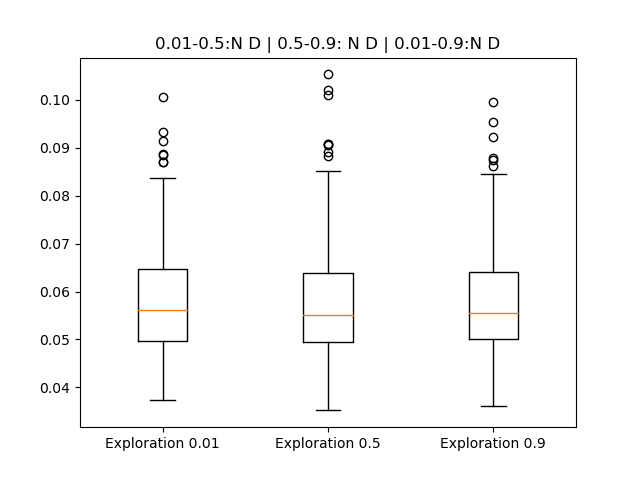
\includegraphics[width = 0.45\textwidth]{Fro_.01-.5-.9pexp_moy_gl.png}
    \end{tabular}
\end{frame}

%-----------------------------------

% Comparer les 3 algorithmes
\begin{frame}
    \frametitle{Tous les algorithmes}
    \begin{tabular}{c c}
        Couverture (volume) & Précision (distance liste but)
        \\
        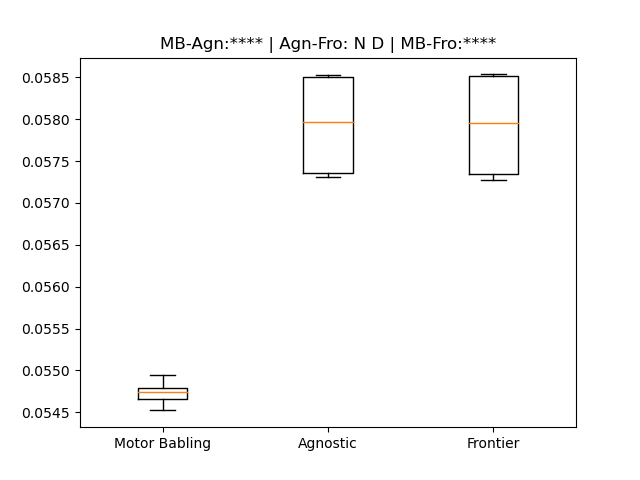
\includegraphics[width = 0.45\textwidth]{ALL_couver.png} &
        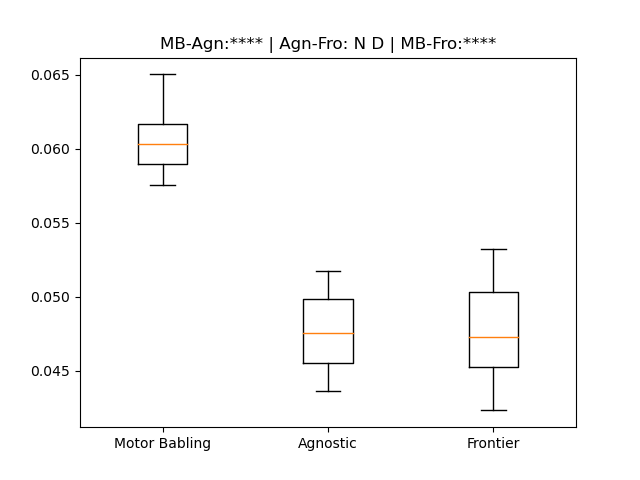
\includegraphics[width = 0.45\textwidth]{ALL_moy_gl.png}
    \end{tabular}
\end{frame}

%###################################
\section{Conclusion}

% Conclusion
\begin{frame}
    % Le but du stage est de calculer la cinématique inverse pour le Poppy Ergo Jr.
    % J'ai tuilisé la méthode de Babling pour la calculer.
    % Pour cela, j'ai testé trois algorithmes. Le motor babling, qui consiste à générer une pose aléatoire, nous donne une couverture moyenne mais une bonne précision
    % Ensuite il y a l'Agnostic Goal Generator, où un but est généré dans la portée du catalogue. Celui-ci nous donne une bonne couverture
    % Enfin, il y a l'algorithme Frontier, qui après discrétisation de l'espace, recherche les cellules à la frontière de la portée du catalogue. C'est ici que j'ai les meilleurs résultats.

    % Les résultats ne sont pas utilisables sur le robot, car les contraintes physiques ont été ignorés. Le robot peut, lors de l'apprentissage, se traverser lui-même. 

    % J'ai choisi le Master AVR par passion pour les matières qui y sont enseginées, et pour découvrir le monde de la recherche. Je suis donc satisfait de ce stage, avec un sujet et un robot que je trouve intéressant, qui permet de conclure ces années d'étude.

    \begin{itemize}
        \item Cinématique Inverse pour Poppy
        \item babling
        \begin{itemize}
            \item Motor Babling
            \item Agnostic Goal Generator
            \item Frontier
        \end{itemize}
        \item Résultats
    \end{itemize}

    % Rappeller le problème: calculer la cinématique inverse pour le poppy
    % Utilisation de l'algorithme du babling
    % Tester les 3 variantes expérience
        % Expliquer Motor babling, couverture & précision
        % Expliquer Agnostique, couverture & précision
        % Expliquer Frontier, couverture & précision
    % Comparaison des 3
\end{frame}

\begin{frame}
    \center
    \Huge Merci de votre attention
    
    Avez-vous des questions ?
\end{frame}

\end{document}